% Options for packages loaded elsewhere
\PassOptionsToPackage{unicode}{hyperref}
\PassOptionsToPackage{hyphens}{url}
\documentclass[
  ignorenonframetext,
]{beamer}
\newif\ifbibliography
\usepackage{pgfpages}
\setbeamertemplate{caption}[numbered]
\setbeamertemplate{caption label separator}{: }
\setbeamercolor{caption name}{fg=normal text.fg}
\beamertemplatenavigationsymbolsempty
% remove section numbering
\setbeamertemplate{part page}{
  \centering
  \begin{beamercolorbox}[sep=16pt,center]{part title}
    \usebeamerfont{part title}\insertpart\par
  \end{beamercolorbox}
}
\setbeamertemplate{section page}{
  \centering
  \begin{beamercolorbox}[sep=12pt,center]{section title}
    \usebeamerfont{section title}\insertsection\par
  \end{beamercolorbox}
}
\setbeamertemplate{subsection page}{
  \centering
  \begin{beamercolorbox}[sep=8pt,center]{subsection title}
    \usebeamerfont{subsection title}\insertsubsection\par
  \end{beamercolorbox}
}
% Prevent slide breaks in the middle of a paragraph
\widowpenalties 1 10000
\raggedbottom
\AtBeginPart{
  \frame{\partpage}
}
\AtBeginSection{
  \ifbibliography
  \else
    \frame{\sectionpage}
  \fi
}
\AtBeginSubsection{
  \frame{\subsectionpage}
}
\usepackage{iftex}
\ifPDFTeX
  \usepackage[T1]{fontenc}
  \usepackage[utf8]{inputenc}
  \usepackage{textcomp} % provide euro and other symbols
\else % if luatex or xetex
  \usepackage{unicode-math} % this also loads fontspec
  \defaultfontfeatures{Scale=MatchLowercase}
  \defaultfontfeatures[\rmfamily]{Ligatures=TeX,Scale=1}
\fi
\usepackage{lmodern}
\ifPDFTeX\else
  % xetex/luatex font selection
\fi
% Use upquote if available, for straight quotes in verbatim environments
\IfFileExists{upquote.sty}{\usepackage{upquote}}{}
\IfFileExists{microtype.sty}{% use microtype if available
  \usepackage[]{microtype}
  \UseMicrotypeSet[protrusion]{basicmath} % disable protrusion for tt fonts
}{}
\makeatletter
\@ifundefined{KOMAClassName}{% if non-KOMA class
  \IfFileExists{parskip.sty}{%
    \usepackage{parskip}
  }{% else
    \setlength{\parindent}{0pt}
    \setlength{\parskip}{6pt plus 2pt minus 1pt}}
}{% if KOMA class
  \KOMAoptions{parskip=half}}
\makeatother
\usepackage{graphicx}
\makeatletter
\newsavebox\pandoc@box
\newcommand*\pandocbounded[1]{% scales image to fit in text height/width
  \sbox\pandoc@box{#1}%
  \Gscale@div\@tempa{\textheight}{\dimexpr\ht\pandoc@box+\dp\pandoc@box\relax}%
  \Gscale@div\@tempb{\linewidth}{\wd\pandoc@box}%
  \ifdim\@tempb\p@<\@tempa\p@\let\@tempa\@tempb\fi% select the smaller of both
  \ifdim\@tempa\p@<\p@\scalebox{\@tempa}{\usebox\pandoc@box}%
  \else\usebox{\pandoc@box}%
  \fi%
}
% Set default figure placement to htbp
\def\fps@figure{htbp}
\makeatother
% definitions for citeproc citations
\NewDocumentCommand\citeproctext{}{}
\NewDocumentCommand\citeproc{mm}{%
  \begingroup\def\citeproctext{#2}\cite{#1}\endgroup}
\makeatletter
 % allow citations to break across lines
 \let\@cite@ofmt\@firstofone
 % avoid brackets around text for \cite:
 \def\@biblabel#1{}
 \def\@cite#1#2{{#1\if@tempswa , #2\fi}}
\makeatother
\newlength{\cslhangindent}
\setlength{\cslhangindent}{1.5em}
\newlength{\csllabelwidth}
\setlength{\csllabelwidth}{3em}
\newenvironment{CSLReferences}[2] % #1 hanging-indent, #2 entry-spacing
 {\begin{list}{}{%
  \setlength{\itemindent}{0pt}
  \setlength{\leftmargin}{0pt}
  \setlength{\parsep}{0pt}
  % turn on hanging indent if param 1 is 1
  \ifodd #1
   \setlength{\leftmargin}{\cslhangindent}
   \setlength{\itemindent}{-1\cslhangindent}
  \fi
  % set entry spacing
  \setlength{\itemsep}{#2\baselineskip}}}
 {\end{list}}
\usepackage{calc}
\newcommand{\CSLBlock}[1]{\hfill\break\parbox[t]{\linewidth}{\strut\ignorespaces#1\strut}}
\newcommand{\CSLLeftMargin}[1]{\parbox[t]{\csllabelwidth}{\strut#1\strut}}
\newcommand{\CSLRightInline}[1]{\parbox[t]{\linewidth - \csllabelwidth}{\strut#1\strut}}
\newcommand{\CSLIndent}[1]{\hspace{\cslhangindent}#1}
\setlength{\emergencystretch}{3em} % prevent overfull lines
\providecommand{\tightlist}{%
  \setlength{\itemsep}{0pt}\setlength{\parskip}{0pt}}
\usepackage{bookmark}
\IfFileExists{xurl.sty}{\usepackage{xurl}}{} % add URL line breaks if available
\urlstyle{same}
% fallback for those not using the hyperref driver hyperxmp:
\makeatletter
\@ifundefined{xmpquote}{\newcommand{\xmpquote}[1]{#1}}{}
\makeatother
\hypersetup{
  pdftitle={Ethical research should be credible research: Do researchers comply with the Declaration of Helsinki?},
  pdfauthor={Cristian Mesquida},
  hidelinks,
  pdfcreator={LaTeX via pandoc}}

\title{\texorpdfstring{Ethical research should be credible research: Do
researchers comply with the Declaration of
Helsinki?}{Ethical research should be credible research: Do researchers comply with the Declaration of Helsinki?}}
\author{\texorpdfstring{Cristian Mesquida}{Cristian Mesquida}}
\date{2025-09-18}
\institute{Eindhoven University of Technology}

\begin{document}
\frame{\titlepage}

\begin{frame}{Discussion points}
\protect\phantomsection\label{discussion-points}
\begin{itemize}
\item
  Declaration of Helsinki
\item
  Informative research vs.~research waste
\item
  Types of research waste
\item
  Reasons for research waste
\item
  Potential solutions
\end{itemize}
\end{frame}

\begin{frame}{Declaration of Helsinki: What it is}
\protect\phantomsection\label{declaration-of-helsinki-what-it-is}
\begin{itemize}
\item
  The Declaration was developed in 1964 by the World Medical Association
\item
  It serves as the international benchmark for ethical conduct in human
  research, providing high-level principles that guide regulatory
  bodies, research institutions, and individual researchers
\end{itemize}

\begin{block}{}
\protect\phantomsection\label{section}
How many of you do know the content of the Declaration of Helsinki?
\end{block}

\begin{block}{}
\protect\phantomsection\label{section-1}
How many of you have declared to adhere to the Declaration of Helsinki?
\end{block}
\end{frame}

\begin{frame}{Declaration of Helsinki 2013}
\protect\phantomsection\label{declaration-of-helsinki-2013}
\textbf{12.} Medical research involving human subjects must be conducted
only by individuals with the appropriate ethics and scientific
education, training and qualifications. Research on patients or healthy
volunteers requires the supervision of a competent and appropriately
qualified physician or other health care professional (World Medical
Association 2013)
\end{frame}

\begin{frame}{Declaration of Helsinki 2013}
\protect\phantomsection\label{declaration-of-helsinki-2013-1}
\textbf{21.} Medical research involving human subjects must conform to
generally accepted scientific principles, be based on a thorough
knowledge of the scientific literature, other relevant sources of
information, and adequate laboratory and, as appropriate, animal
experimentation. {[}\ldots{]} (World Medical Association 2013)
\end{frame}

\begin{frame}{Declaration of Helsinki 2024}
\protect\phantomsection\label{declaration-of-helsinki-2024}
\textbf{21.} Medical research involving human participants must have a
scientifically sound and rigorous design and execution that are likely
to produce reliable, valid, and valuable knowledge and avoid
\textbf{research waste} {[}\ldots{]} (World Medical Association 2025)
\end{frame}

\begin{frame}{Declaration of Helsinki 2024}
\protect\phantomsection\label{declaration-of-helsinki-2024-1}
\textbf{36.} Researchers, authors, sponsors, editors, and publishers all
have ethical obligations with regard to the publication and
dissemination of the results of research. Researchers have a duty to
make publicly available the results of their research on human
participants and are accountable for the timeliness, completeness, and
accuracy of their reports. All parties should adhere to accepted
guidelines for ethical reporting. Negative and inconclusive as well as
positive results must be published or otherwise made publicly available
(World Medical Association 2025)
\end{frame}

\begin{frame}{Informative research}
\protect\phantomsection\label{informative-research}
\begin{itemize}
\item
  The process of gathering and analyzing data to produce trustworthy
  knowledge
\item
  It is carried out through ethical and rigorous methods, and
  communicated transparently and without bias, enabling peers to verify
  and build upon the findings
\end{itemize}
\end{frame}

\begin{frame}{Why do we do research?}
\protect\phantomsection\label{why-do-we-do-research}
\begin{itemize}
\item
  To test the the efficacy/effectiveness of interventions
\item
  Is intervention A more effective than intervention B in reducing time
  to return-to-play in football players after injury?
\end{itemize}
\end{frame}

\begin{frame}{Research waste}
\protect\phantomsection\label{research-waste}
Research that fails to produce reliable or relevant results that cannot
be be used to inform decision making
\end{frame}

\begin{frame}{Research waste}
\protect\phantomsection\label{research-waste-1}
\begin{center}
\includegraphics[width=0.7\linewidth]{figures/fig1} \end{center}

(Altman 1994)
\end{frame}

\begin{frame}{Waste at four stages of research}
\protect\phantomsection\label{waste-at-four-stages-of-research}
Question -\textgreater{} Design and analysis -\textgreater{} Reporting
-\textgreater{} Publication
\end{frame}

\begin{frame}{1-Research question}
\protect\phantomsection\label{research-question}
\begin{itemize}
\item
  Irrelevant/low priority questions addressed
\item
  Redundancy
\end{itemize}
\end{frame}

\begin{frame}{Example: Cumulative Meta-Analysis of Therapeutic Trials
for Myocardial Infarction (Lau et al. 1992)}
\protect\phantomsection\label{example-cumulative-meta-analysis-of-therapeutic-trials-for-myocardial-infarction-lau_cumulative_1992}
\begin{itemize}
\item
  Thirty-three trials evaluating this therapy were performed between
  1959 and 1988
\item
  Statistically significant reduction in mortality (odds ratio, 0.74;
  95\% CI {[}0.59 to 0.92{]}) was achieved in 1973, after only eight
  trials involving 2432 patients
\item
  The results of the 25 subsequent trials (34,542 additional patients)
  through 1988 had little or no effect on the odds ratio establishing
  efficacy, but simply narrowed the 95\% CI
\item
  Two very large trials in 1986 (11,712 patients) and in 1988 (17,187
  patients) did not modify the already established evidence of efficacy
\end{itemize}
\end{frame}

\begin{frame}{Cumulative Meta-Analysis of Therapeutic Trials for
Myocardial Infarction}
\protect\phantomsection\label{cumulative-meta-analysis-of-therapeutic-trials-for-myocardial-infarction}
\begin{center}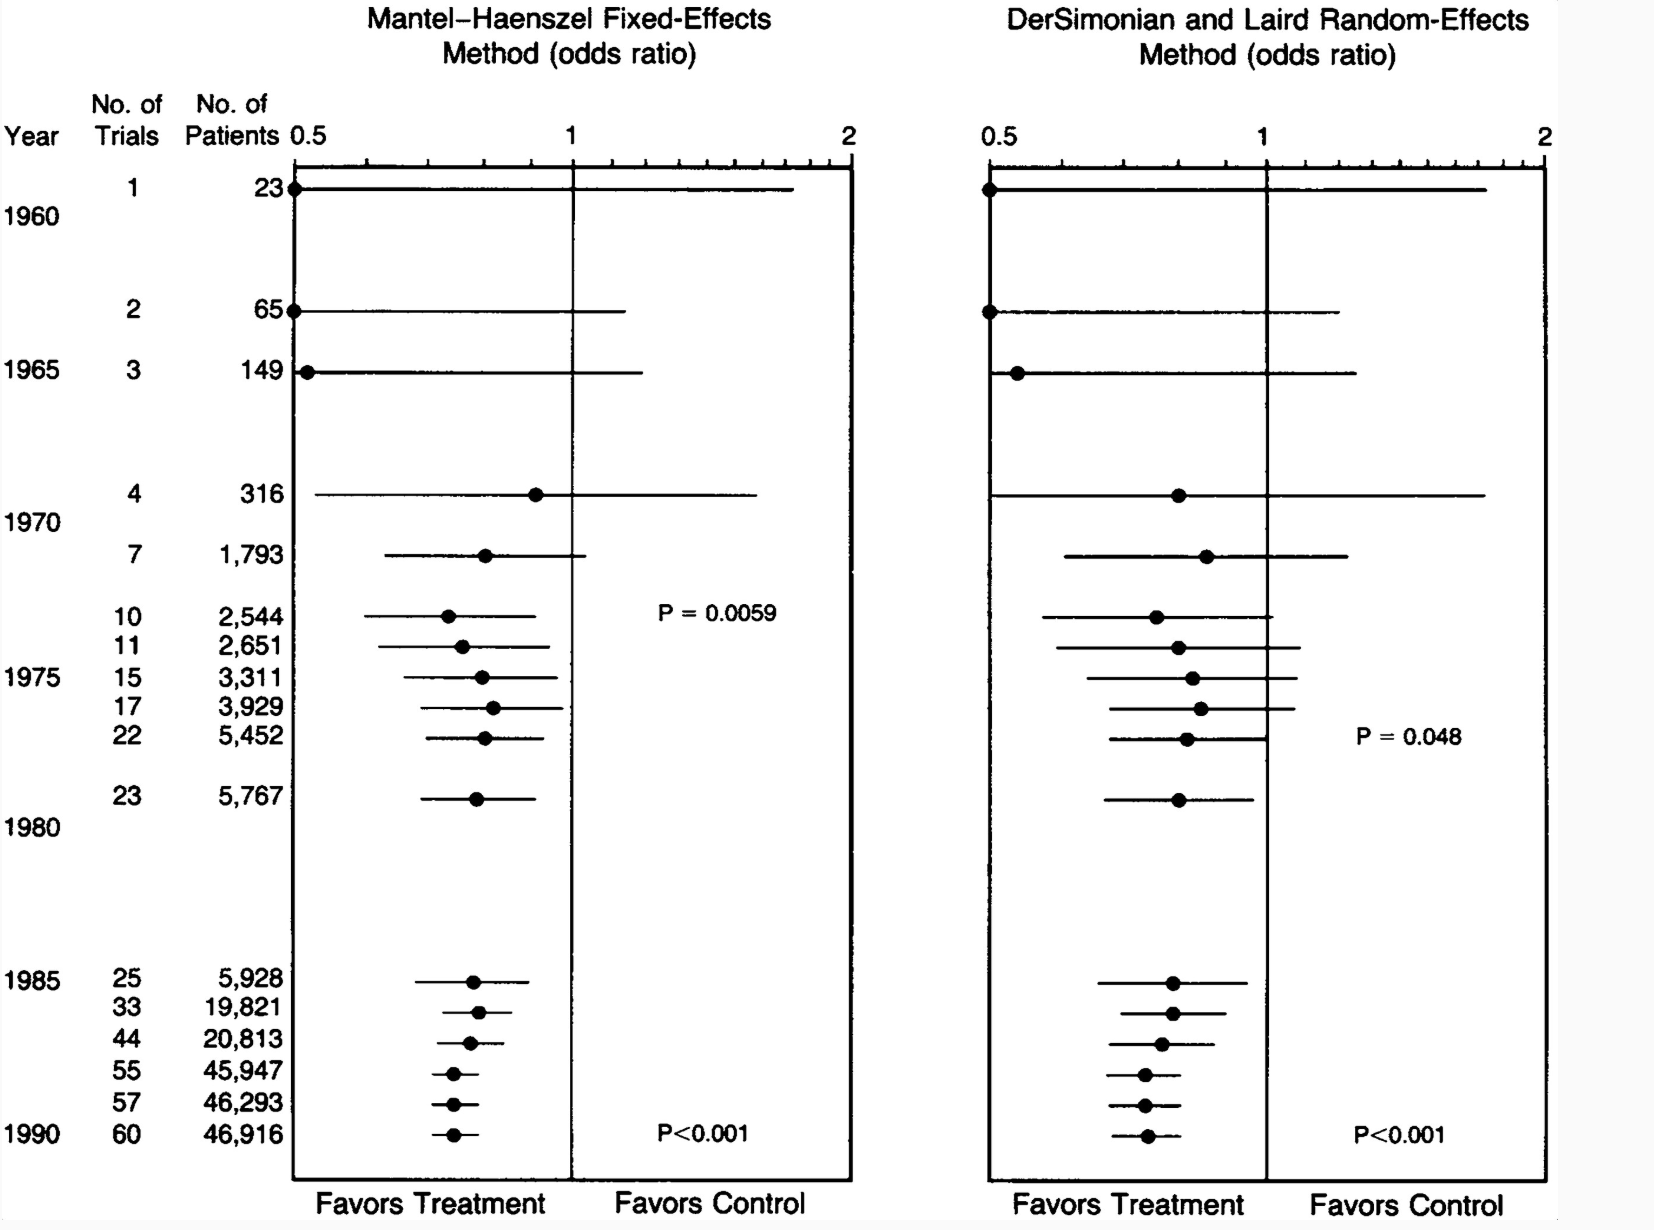
\includegraphics[width=0.8\linewidth]{figures/fig2} \end{center}

(Lau et al. 1992)
\end{frame}

\begin{frame}{Example in sports and exercise science: The effect of
self-talk interventions on sports/motor performance}
\protect\phantomsection\label{example-in-sports-and-exercise-science-the-effect-of-self-talk-interventions-on-sportsmotor-performance}
\begin{itemize}
\item
  Since Hatzigeorgiadis et al. (2011) meta-analysis the number of
  studies conducted examining the effects of self-talk interventions on
  sport/motor performance has roughly doubled
\item
  35 new studies published from November 2011 up to November 2023
\item
  The overall effect in Hatzigeorgiadis et al. (2011) was 0.48 95\% CI
  (0.38; 0.58) and after adding newer studies the overall effect was
  0.47 95\% CI (0.39; 0.56) in Corcoran and Steele (2024)
\end{itemize}
\end{frame}

\begin{frame}{Relevant research question}
\protect\phantomsection\label{relevant-research-question}
New research should be set in the context of an evidence gap and should
involve stakeholders when possible
\end{frame}

\begin{frame}{2- Study design}
\protect\phantomsection\label{study-design}
Conduct studies that do not answer the research question (Mesquida et
al. 2025d). For instance:

\begin{itemize}
\item
  23 out of 350 studies tested a hypothesis of equivalence using a
  classic null hypothesis test (Mesquida et al. 2025a)
\item
  Testing for treatment effects by separate analyses of changes from
  baseline in each group is a misleading approach
\end{itemize}

\begin{center}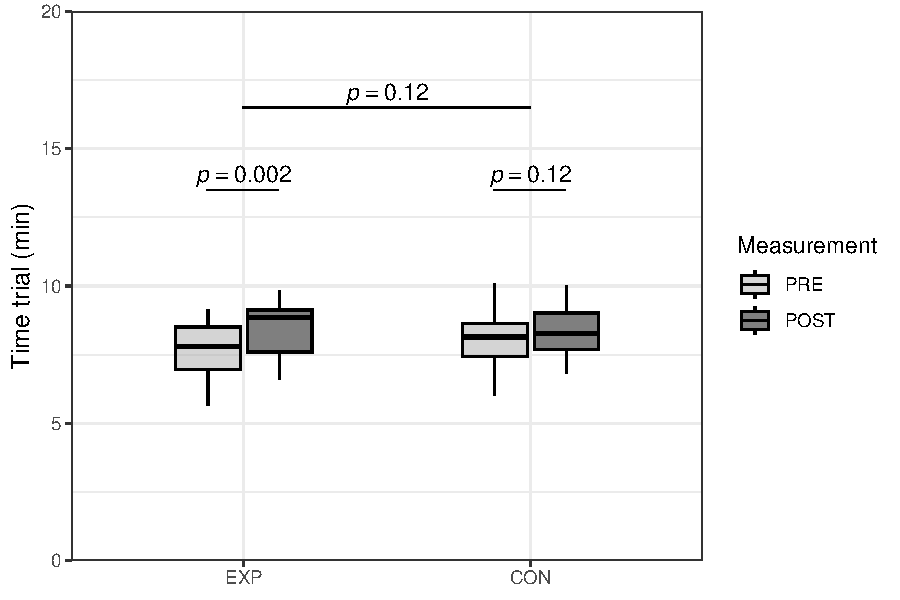
\includegraphics[width=0.6\linewidth]{figures/fig10} \end{center}
\end{frame}

\begin{frame}{2- Study design}
\protect\phantomsection\label{study-design-1}
Invalid a priori power analyses (Mesquida et al. 2025b):

\begin{itemize}
\item
  Mean sample size of \textasciitilde{} 30 participants
\item
  40\% (139 out of 350) of hypothesis-testing studies reported
  conducting an a priori power analysis.
\item
  No significant difference in sample size between studies that reported
  an a priori power analyses and those that did not
\item
  No significant difference in the proportion of hypotheses supported
  between studies that reported an a priori power analyses and those
  that did not
\item
  Potential reasons: sample size bamba (Schulz and Grimes 2005), invalid
  effect sizes, inflated effect sizes
\end{itemize}
\end{frame}

\begin{frame}{How a power analysis implicitly reveals the smallest
effect size you care about}
\protect\phantomsection\label{how-a-power-analysis-implicitly-reveals-the-smallest-effect-size-you-care-about}
\begin{center}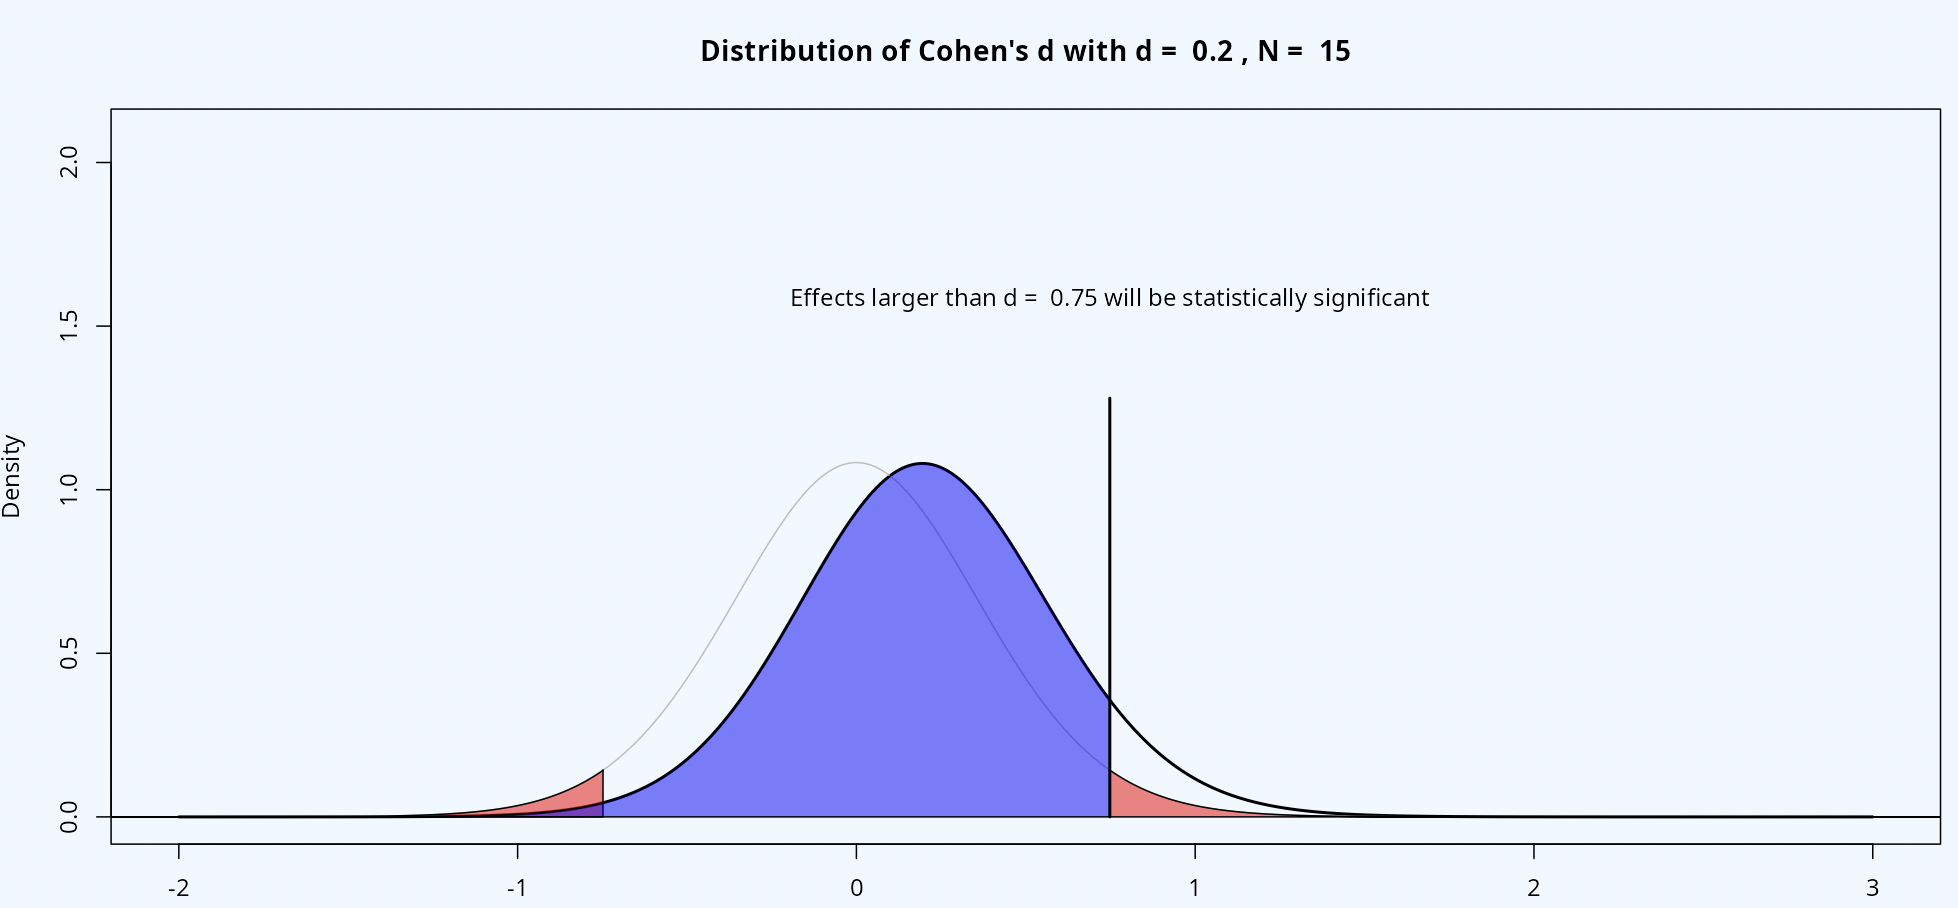
\includegraphics[width=0.8\linewidth]{figures/fig3} \end{center}
\end{frame}

\begin{frame}{2- Study design}
\protect\phantomsection\label{study-design-2}
\begin{itemize}
\item
  \textbf{Low statistical power}: an analysis of 269 hypothesis-testing
  studies showed that the average statistical power was 11\% (Mesquida
  et al. 2025a)
\item
  \textbf{Implication}: With such low power, the chance of detecting
  true effects is extremely low
\item
  Flipping a coin (50\% probability).
\end{itemize}
\end{frame}

\begin{frame}{Why designing studies with high statistical power is
important?}
\protect\phantomsection\label{why-designing-studies-with-high-statistical-power-is-important}
1- Interpretation of null findings

\begin{itemize}
\tightlist
\item
  If a study is designed with low power (e.g., 20\%), a null significant
  result cannot be interpreted because it could be due to that the
  effect size is smaller than expected or non-existent.
\end{itemize}
\end{frame}

\begin{frame}{Why designing studies with high statistical power is
important?}
\protect\phantomsection\label{why-designing-studies-with-high-statistical-power-is-important-1}
2- Narrower confidence intervals

\begin{itemize}
\item
  Example 1: study with 20 participants yields a wider 95\% CI {[}-0.72;
  1.16{]}
\item
  Example 2: study with 200 participants yields a narrower 95\% CI
  {[}-0.75; -0.23{]}
\end{itemize}
\end{frame}

\begin{frame}{2- Study design}
\protect\phantomsection\label{study-design-3}
Lack of transparency

\begin{itemize}
\item
  Framing your study as confirmatory when is exploratory (Ditroilo et
  al. 2025)
\item
  Vague and unfalsifiable hypotheses (Mesquida et al. 2025d)
\end{itemize}
\end{frame}

\begin{frame}{3- Selection bias}
\protect\phantomsection\label{selection-bias}
\begin{itemize}
\item
  Publication bias
\item
  Flexibility in data analysis
\end{itemize}

\begin{center}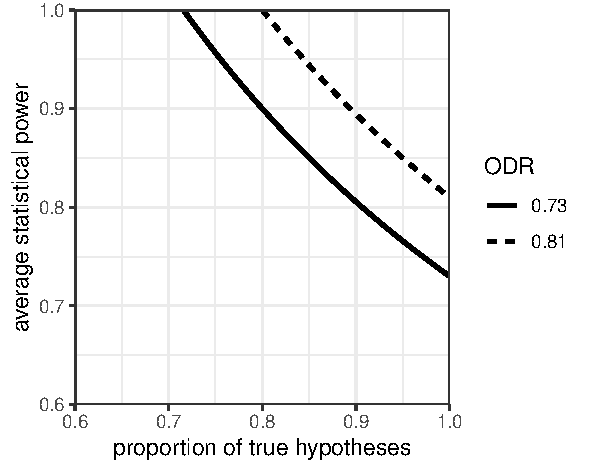
\includegraphics[width=0.6\linewidth]{figures/fig4} \end{center}

(Mesquida et al. 2025a)
\end{frame}

\begin{frame}{Publication bias}
\protect\phantomsection\label{publication-bias}
\begin{center}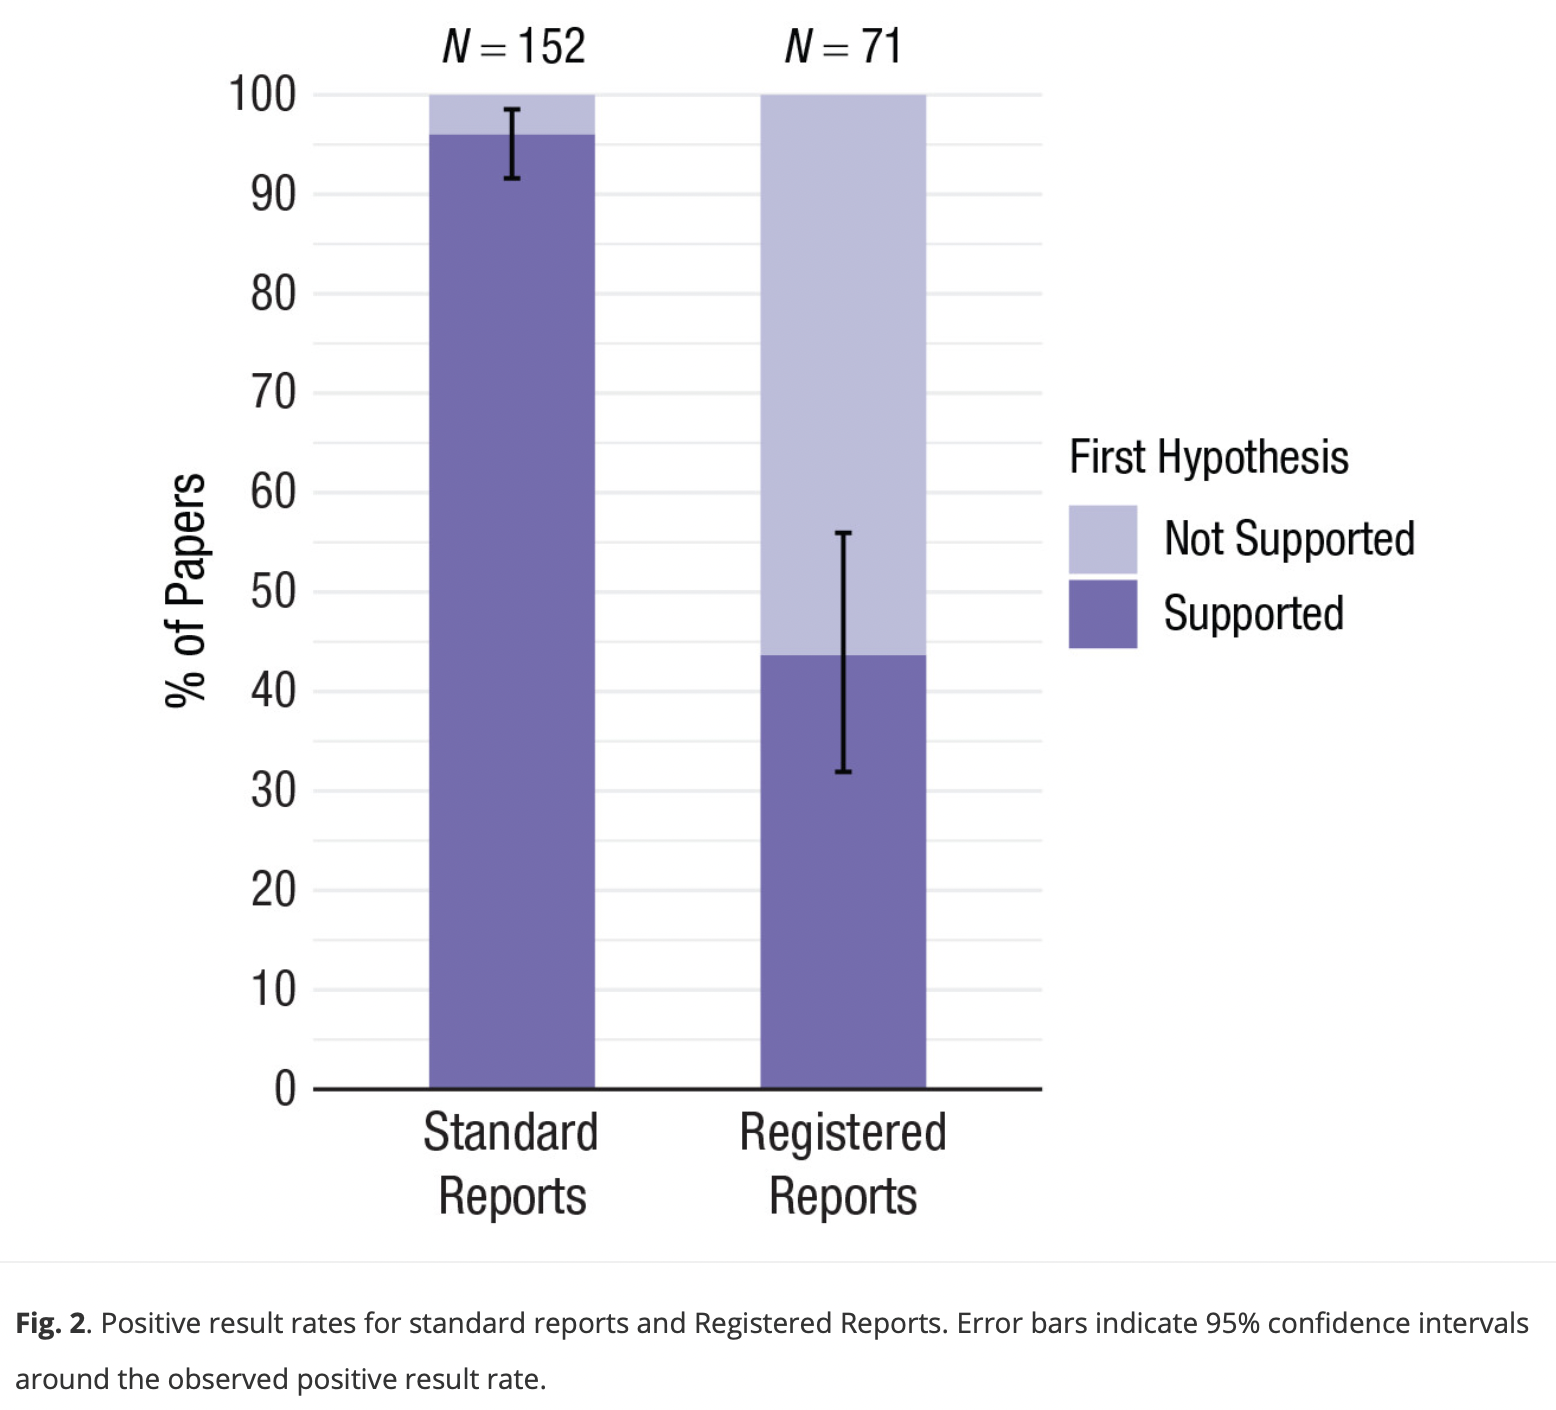
\includegraphics[width=0.6\linewidth]{figures/fig5} \end{center}

(Scheel et al. 2021)
\end{frame}

\begin{frame}{Flexibility in data analysis}
\protect\phantomsection\label{flexibility-in-data-analysis}
\begin{figure}

{\centering 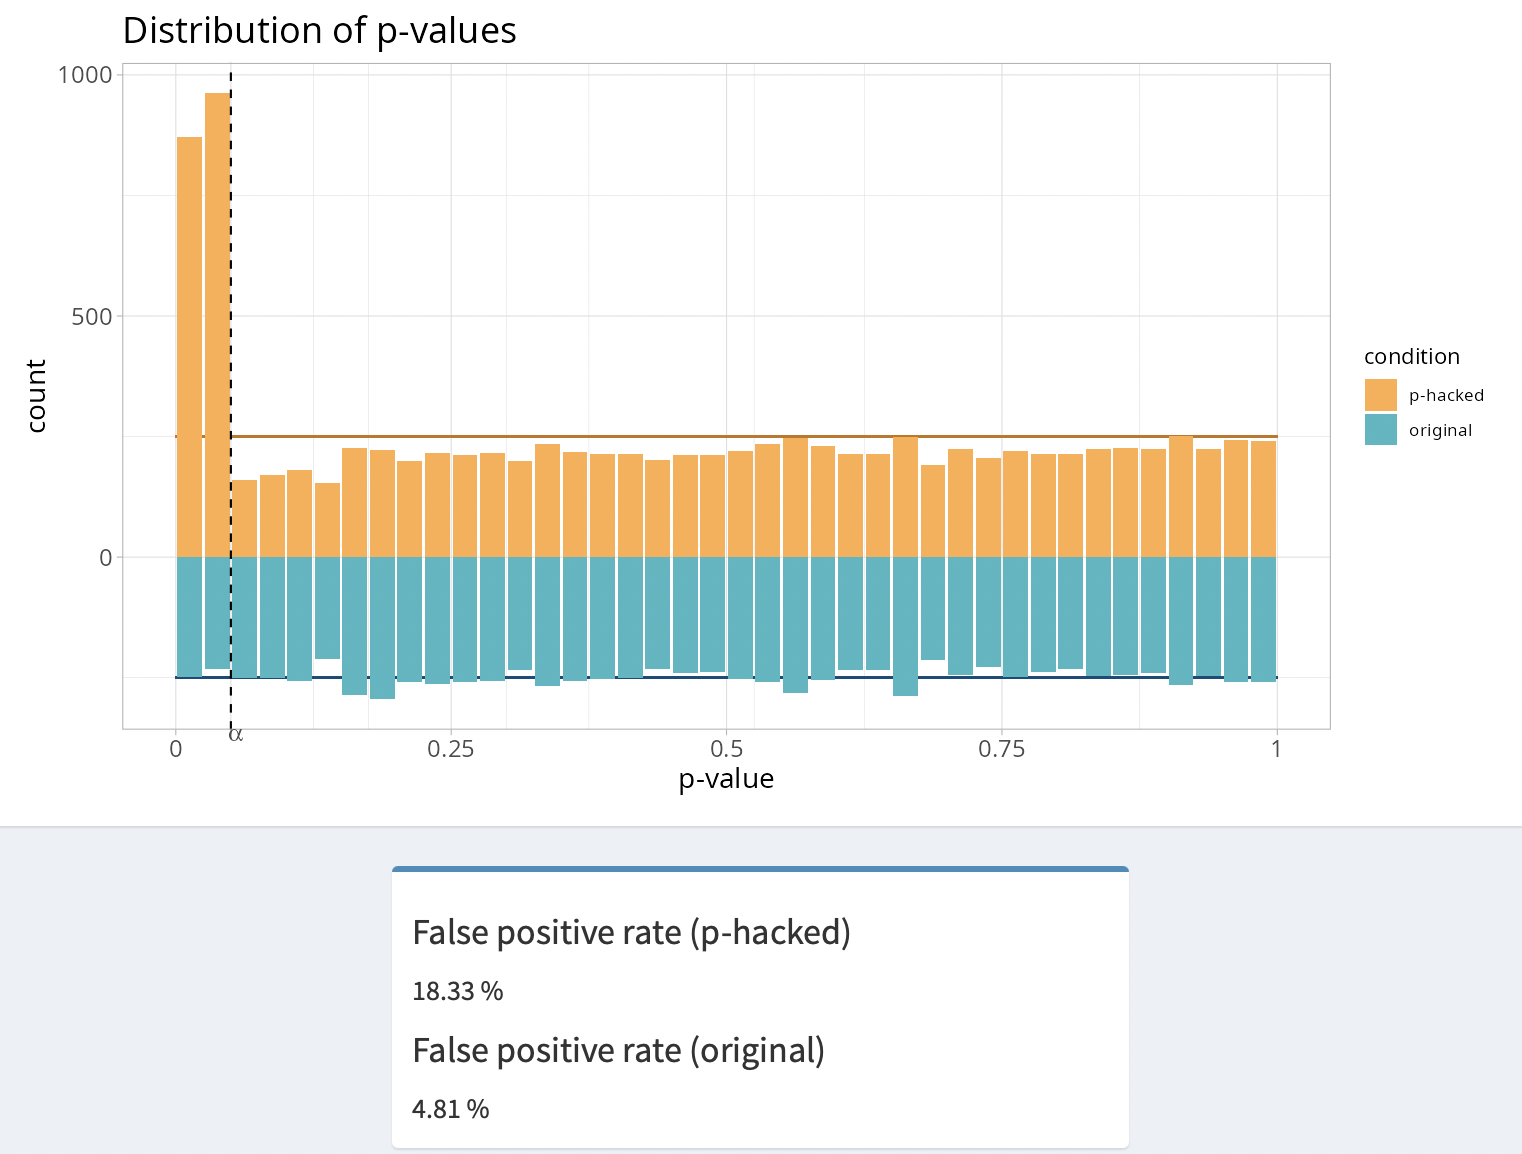
\includegraphics[width=0.6\linewidth]{figures/fig6} 

}

\caption{Distribution of effect sizes under the null hypothesis when performing 5 indepdendent t-tests, the correlation between dependent variables is 0.5 and alpha level is 0.05}\label{fig:unnamed-chunk-8}
\end{figure}
\end{frame}

\begin{frame}{Selection bias and statistical power in sports and
exercise science}
\protect\phantomsection\label{selection-bias-and-statistical-power-in-sports-and-exercise-science}
\begin{center}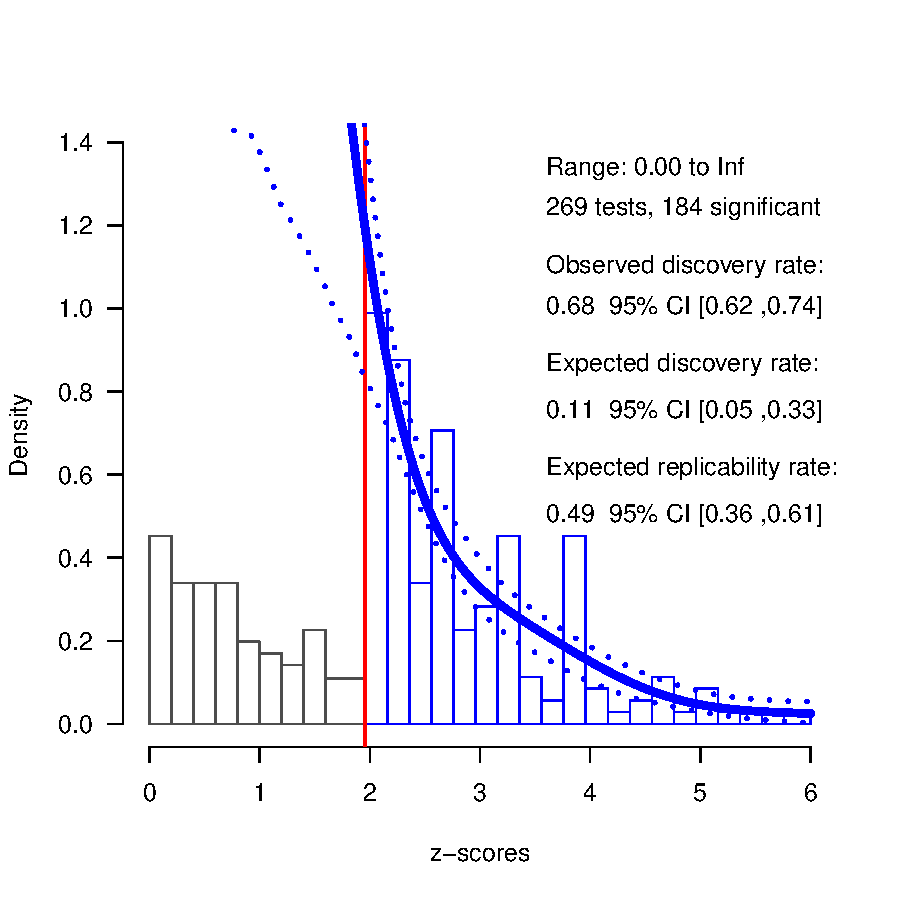
\includegraphics[width=0.6\linewidth]{figures/fig7} \end{center}

(Mesquida et al. 2025a)
\end{frame}

\begin{frame}{Consequences of selection bias and studies with
underpowered designs}
\protect\phantomsection\label{consequences-of-selection-bias-and-studies-with-underpowered-designs}
\begin{center}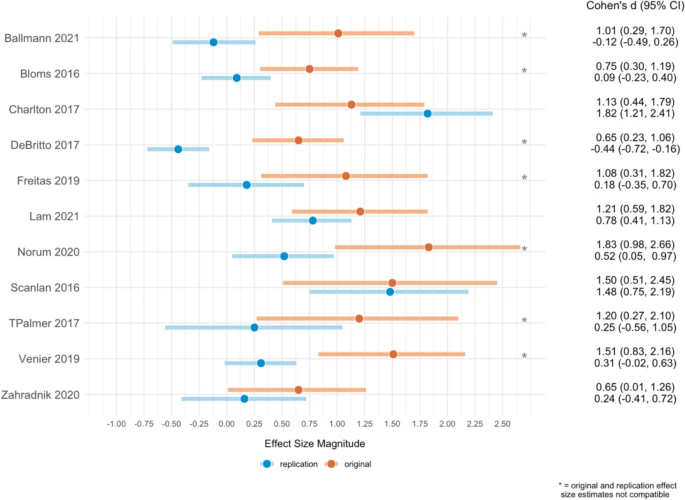
\includegraphics[width=0.7\linewidth]{figures/fig8} \end{center}

({Murphy, Caldwell, Mesquida, et al.} 2025)
\end{frame}

\begin{frame}{Results of the Sports Science Replication Project
({Murphy, Caldwell, Mesquida, et al.} 2025)}
\protect\phantomsection\label{results-of-the-sports-science-replication-project-murphy_replicability_2025}
\begin{itemize}
\item
  Inflated type I error rate: 56\% of the 25 analysed replication
  studies had a statistically significant p-value similar to the
  original studies
\item
  Inflated effect sizes: median percentage decrease in magnitude from
  the original to the replication effect size estimate equal to 75\% for
  all of the replication effect sizes
\item
  Only 36\% of replication and original effect size estimates were
  compatible
\end{itemize}
\end{frame}

\begin{frame}{Results from other meta-scientific studies}
\protect\phantomsection\label{results-from-other-meta-scientific-studies}
\begin{center}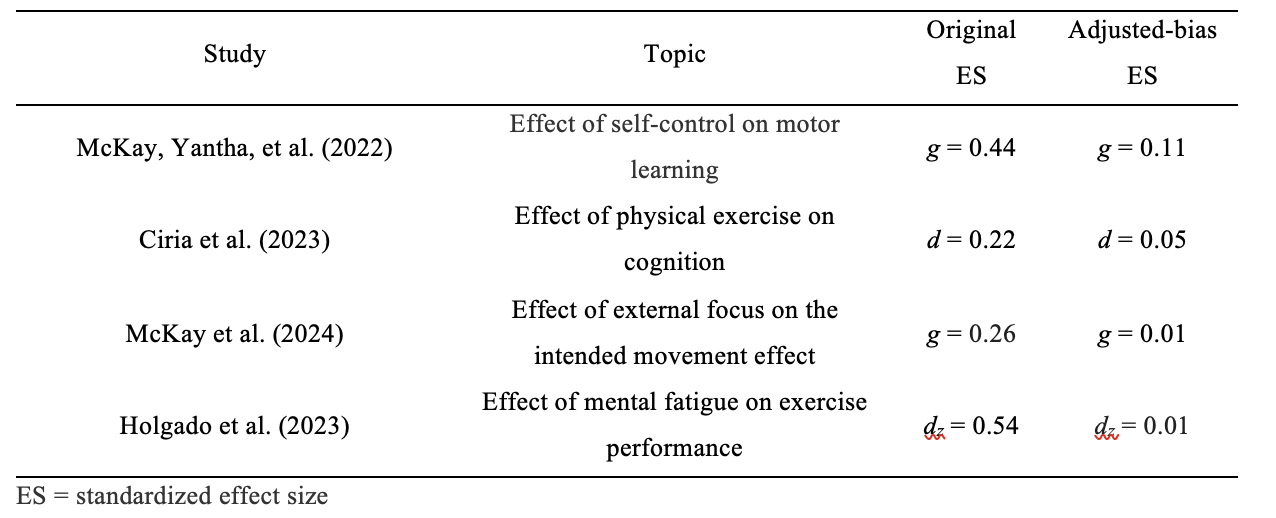
\includegraphics[width=0.9\linewidth]{figures/table1} \end{center}
\end{frame}

\begin{frame}{4- Reporting of statistical information and data sharing}
\protect\phantomsection\label{reporting-of-statistical-information-and-data-sharing}
\begin{itemize}
\item
  ``This project faced many practical challenges when preparing studies
  for replication, specifically the poor reporting of statistical
  information, the availability of original raw data {[}\ldots{]}''
  (Murphy, Caldwell, and Warne 2025)
\item
  Out of 350 hypothesis-testing hypotheses, 57\% (46/81) could not be
  recomputed into an exact p-value due to poor reporting of statistical
  information or availability of original raw data (Mesquida et al.
  2025a)
\end{itemize}
\end{frame}

\begin{frame}{4- Reporting of statistics and data sharing}
\protect\phantomsection\label{reporting-of-statistics-and-data-sharing}
\begin{center}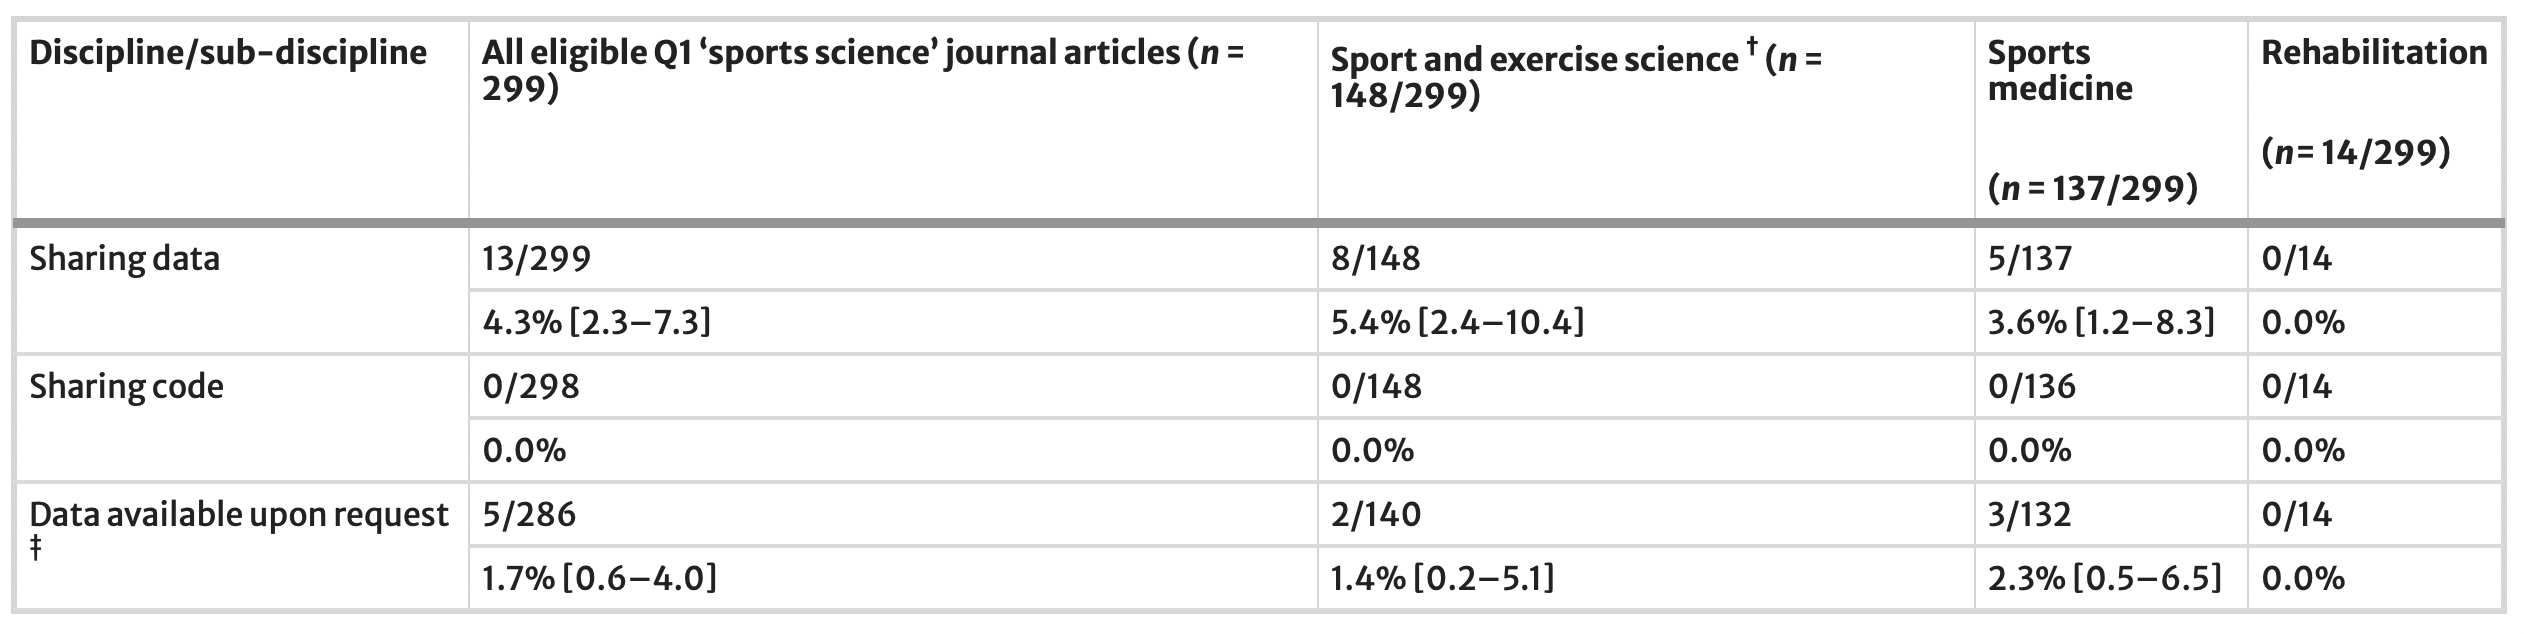
\includegraphics[width=1\linewidth]{figures/table2} \end{center}

(Borg et al. 2020)
\end{frame}

\begin{frame}{Why sharing data and code are important?}
\protect\phantomsection\label{why-sharing-data-and-code-are-important}
\begin{itemize}
\item
  Verify results: Allow peers to reproduce and confirm the findings
\item
  Reuse data: Facilitate meta-analyses, replications, secondary
  analyses, or new research projects
\item
  Increase transparency: Promote trust and accountability in research
\end{itemize}
\end{frame}

\begin{frame}{Research waste also affect meta-analyses}
\protect\phantomsection\label{research-waste-also-affect-meta-analyses}
In the 30 most cited meta-analyses in S\&C research, Kadlec et al.
(2023) found that:

\begin{itemize}
\item
  Almost 45\% contained at least one effect size that was mistakenly
  calculated using SE rather than SD.
\item
  45\% failed to account for effect size dependency
\end{itemize}

In 96 meta-analyses published in Sports Medicine, Mesquida et al.
(2025c) found that:

\begin{itemize}
\item
  16\% of 96 meta-analyses contained data to reproduce study effect
  sizes
\item
  Many combined studies with different designs (e.g., within- and
  between-designs, RCT and non-RCT)
\item
  34\% did not account for effect size dependency
\end{itemize}
\end{frame}

\begin{frame}{Summary}
\protect\phantomsection\label{summary}
\begin{itemize}
\item
  Research waste in the form of studies that do not answer the research
  question, inflated effect sizes, study designs with low power, poor
  reporting of statistical practices and lack of data sharing and low
  methodligical quality of meta-analyses
\item
  We, as a community, are not properly trained to conduct informative
  research
\end{itemize}
\end{frame}

\begin{frame}{Drivers of research waste}
\protect\phantomsection\label{drivers-of-research-waste}
Wrong incentives:

\begin{itemize}
\item
  Quantity vs.~quality: mass produce sports and exercise science
  research for career purposes
\item
  Preference for studies that report positive findings
\item
  Compete for limited resources
\end{itemize}
\end{frame}

\begin{frame}{Drivers of research waste}
\protect\phantomsection\label{drivers-of-research-waste-1}
\begin{itemize}
\item
  Time constraints: lack of time to develop expertise and skills
\item
  Incompetence: insufficient training
\end{itemize}
\end{frame}

\begin{frame}{How to avoid research waste}
\protect\phantomsection\label{how-to-avoid-research-waste}
\begin{center}
\includegraphics[width=0.9\linewidth]{figures/fig9} \end{center}
\end{frame}

\begin{frame}{Long-term solutions}
\protect\phantomsection\label{long-term-solutions}
\begin{itemize}
\item
  Reward researchers not for the number of publications but for the
  quality of their research
\item
  More time for improving research competences
\item
  Improve statistical training at BSc and MSc
\end{itemize}
\end{frame}

\begin{frame}{How to avoid research waste}
\protect\phantomsection\label{how-to-avoid-research-waste-1}
Mid-term solutions

\begin{itemize}
\item
  Science as a collaborative effort where each member brings specialized
  expertise
\item
  Big Team Science
\end{itemize}

Question -\textgreater{} Design -\textgreater{} Analysis Plan
-\textgreater{} Data collection -\textgreater{} Analysis execution
-\textgreater{} Reporting -\textgreater{} Interpretation -\textgreater{}
Data stewardship
\end{frame}

\begin{frame}{Science as a collaborative effort}
\protect\phantomsection\label{science-as-a-collaborative-effort}
\begin{itemize}
\item
  The goal is not to conduct experiments alone or with small group of
  collaborators which may lack expertise in some areas
\item
  The goal is to support and ehance collective scientific research
\end{itemize}
\end{frame}

\begin{frame}{Science as a collaborative effort}
\protect\phantomsection\label{science-as-a-collaborative-effort-1}
\begin{itemize}
\tightlist
\item
  Theorists -\textgreater{} develop frameworks or hypotheses to explain
  phenomena
\item
  Methodologists -\textgreater{} statisticians -\textgreater design
  studies and slect appropiate methods
\item
  Data collectors -\textgreater{} gather and organize raw data
\item
  Experts in interpreting effect sizes -\textgreater{} assess the
  practical significance of findings
\item
  Data stewards -\textgreater{} manage, curate and maintain datasets to
  ensure FAIR principles and reproducibility
\end{itemize}
\end{frame}

\begin{frame}{Specialization}
\protect\phantomsection\label{specialization}
\begin{itemize}
\tightlist
\item
  \textbf{12}. Medical research involving human participants must be
  conducted only by individuals with the appropriate ethics and
  scientific education, training and qualifications. Such research
  requires the supervision of a competent and appropriately qualified
  physician or other researcher (World Medical Association 2025)
\end{itemize}
\end{frame}

\begin{frame}{How to avoid research waste}
\protect\phantomsection\label{how-to-avoid-research-waste-2}
Short-term solutions

\begin{itemize}
\item
  Collaboration with applied statisticians (Sainani et al. 2021)
\item
  Registered Reports (?)
\end{itemize}
\end{frame}

\begin{frame}[allowframebreaks]{References}
\protect\phantomsection\label{references}
\protect\phantomsection\label{refs}
\begin{CSLReferences}{1}{1}
\bibitem[\citeproctext]{ref-altman_scandal_1994}
Altman, D. G. 1994. {``The Scandal of Poor Medical Research.''}
\emph{British Medical Journal} 308 (6924): 283--84.
\url{https://doi.org/10.1136/bmj.308.6924.283}.

\bibitem[\citeproctext]{ref-borg_sharing_practices}
Borg, David N., Joshua J. Bon, Kristin L. Sainani, Brenton J. Baguley,
Nicholas J. Tierney, and Christopher Drovandi. 2020. {``Comment on:
{`{Moving Sport} and {Exercise Science Forward}: {A Call} for the
{Adoption} of {More Transparent Research Practices}'}.''} \emph{Sports
Medicine} 50 (8): 1551--53.
\url{https://doi.org/10.1007/s40279-020-01298-5}.

\bibitem[\citeproctext]{ref-steele_waste_2024}
Corcoran, Hannah, and James Steele. 2024. \emph{Cumulative Evidence
Synthesis and Consideration of "Research Waste" Using {Bayesian}
Methods: {An} Example Updating a Previous Meta-Analysis of Self-Talk
Interventions for Sport/Motor Performance}. SportRxiv.
\url{https://doi.org/10.51224/SRXIV.348}.

\bibitem[\citeproctext]{ref-ditroilo_exploratory}
Ditroilo, Massimiliano, Cristian Mesquida, Grant Abt, and Daniël Lakens.
2025. {``Exploratory Research in Sport and Exercise Science:
{Perceptions}, Challenges, and Recommendations.''} \emph{Journal of
Sports Sciences}, April, 1--13.
\url{https://doi.org/10.1080/02640414.2025.2486871}.

\bibitem[\citeproctext]{ref-hatzigeorgiadis_2011}
Hatzigeorgiadis, Antonis, Nikos Zourbanos, Evangelos Galanis, and
Yiannis Theodorakis. 2011. {``Self-{Talk} and {Sports Performance}: {A
Meta-Analysis}.''} \emph{Perspectives on Psychological Science} 6 (4):
348--56. \url{https://doi.org/10.1177/1745691611413136}.

\bibitem[\citeproctext]{ref-kadlec_2023}
Kadlec, Daniel, Kristin L. Sainani, and Sophia Nimphius. 2023. {``With
{Great Power Comes Great Responsibility}: {Common Errors} in
{Meta-Analyses} and {Meta-Regressions} in {Strength} \& {Conditioning
Research}.''} \emph{Sports Medicine} 53 (2): 313--25.
\url{https://doi.org/10.1007/s40279-022-01766-0}.

\bibitem[\citeproctext]{ref-lau_cumulative_1992}
Lau, Joseph, Elliott M. Antman, Jeanette Jimenez-Silva, Bruce Kupelnick,
Frederick Mosteller, and Thomas C. Chalmers. 1992. {``Cumulative
{Meta-Analysis} of {Therapeutic Trials} for {Myocardial Infarction}.''}
\emph{New England Journal of Medicine} 327 (4): 248--54.
\url{https://doi.org/10.1056/NEJM199207233270406}.

\bibitem[\citeproctext]{ref-mesquida_zcurve_2025}
Mesquida, Cristian, Jennifer Murphy, Joe Warne, and Daniël Lakens.
2025a. \emph{On the Replicability of Sports and Exercise Science
Research: Assessing the Prevalence of Publication Bias and Studies with
Underpowered Designs by a z-Curve Analysis}. SportRxiv.
\url{https://doi.org/10.51224/SRXIV.534}.

\bibitem[\citeproctext]{ref-mesquida_power_analysis_2025}
Mesquida, Cristian, Jennifer Murphy, Joe Warne, and Daniël Lakens.
2025b. \emph{The Prevalence, Reporting Practices, and Methodological
Quality of a Priori Power Analyses in Sports and Exercise Science
Research}. SportRxiv. \url{https://doi.org/10.51224/SRXIV.575}.

\bibitem[\citeproctext]{ref-mesquida_metaanalyses}
Mesquida, Cristian, Joe Warne, and Daniël Lakens. 2025c. \emph{A Scoping
Review of the Transparency, Reporting Practices and Methodological Rigor
of Meta-Analyses Published in {Sports Medicine}}. SportRxiv.
\url{https://doi.org/10.51224/SRXIV.576}.

\bibitem[\citeproctext]{ref-mesquida_what_is_your_hypo}
Mesquida, Cristian, Joe Warne, and Daniël Lakens. 2025d. \emph{What Is
Your Hypothesis? {On} the Importance of Knowing Your Hypothesis Before
Conducting a Hypothesis Test}. SportRxiv.
\url{https://doi.org/10.51224/SRXIV.577}.

\bibitem[\citeproctext]{ref-murphy_replicability_2025}
{Murphy, Jennifer, Aaron R. Caldwell, Cristian Mesquida, et al.} 2025.
{``Estimating the {Replicability} of {Sports} and {Exercise Science
Research}.''} \emph{Sports Medicine}, ahead of print.
\url{https://doi.org/10.1007/s40279-025-02201-w}.

\bibitem[\citeproctext]{ref-murphy_reflections}
Murphy, Jennifer, Aaron R. Caldwell, and Joe P. Warne. 2025.
{``Reflections on {Conducting} a {Large Replication Project} in {Sports}
and {Exercise Science}.''} \emph{Sports Medicine}, ahead of print, June.
\url{https://doi.org/10.1007/s40279-025-02200-x}.

\bibitem[\citeproctext]{ref-sainani_collaboration}
Sainani, Kristin L., David N. Borg, Aaron R. Caldwell, et al. 2021.
{``Call to Increase Statistical Collaboration in Sports Science, Sport
and Exercise Medicine and Sports Physiotherapy.''} \emph{British Journal
of Sports Medicine} 55 (2): 118--22.
\url{https://doi.org/10.1136/bjsports-2020-102607}.

\bibitem[\citeproctext]{ref-scheel_excessive}
Scheel, Anne M., Mitchell R. M. J. Schijen, and Daniël Lakens. 2021.
{``An {Excess} of {Positive Results}: {Comparing} the {Standard
Psychology Literature With Registered Reports}.''} \emph{Advances in
Methods and Practices in Psychological Science} 4 (2): 1--12.
\url{https://doi.org/10.1177/25152459211007467}.

\bibitem[\citeproctext]{ref-sample_size_bamba}
Schulz, Kenneth F., and David A. Grimes. 2005. {``Sample Size
Calculations in Randomised Trials: Mandatory and Mystical.''} \emph{The
Lancet} 365 (9467): 1348--53.
\url{https://doi.org/10.1016/S0140-6736(05)61034-3}.

\bibitem[\citeproctext]{ref-helsinky_2013}
World Medical Association. 2013. {``World {Medical Association
Declaration} of {Helsinki}: {Ethical Principles} for {Medical Research
Involving Human Subjects}.''} \emph{JAMA} 310 (20): 2191--94.
\url{https://doi.org/10.1001/jama.2013.281053}.

\bibitem[\citeproctext]{ref-helsinky_2025}
World Medical Association. 2025. {``World {Medical Association
Declaration} of {Helsinki}: {Ethical Principles} for {Medical Research
Involving Human Participants}.''} \emph{JAMA} 333 (1): 71--74.
\url{https://doi.org/10.1001/jama.2024.21972}.

\end{CSLReferences}
\end{frame}

\end{document}
